\documentclass[12p,a4paper]{article}
\usepackage[utf8]{inputenc}
\usepackage[T1]{fontenc,url}
\usepackage{multicol}
\usepackage{multirow}
\usepackage{parskip}
\usepackage{lmodern}
\usepackage{microtype}
\usepackage{verbatim}
\usepackage{amsmath, amssymb}
\usepackage{tikz}
\usepackage{physics}
\usepackage{mathtools}
\usepackage{algorithm}
\usepackage{algpseudocode}
\usepackage{listings}
\usepackage{enumerate}
\usepackage{graphicx}
\usepackage{float}
\usepackage{hyperref}
\usepackage{tabularx}
\usepackage{siunitx}
\usepackage{fancyvrb}
\usepackage[makeroom]{cancel}
\usepackage[margin=2.0cm]{geometry}
\renewcommand{\baselinestretch}{1}
\renewcommand{\exp}{e^}
\renewcommand{\b}{\boldsymbol}
\newcommand{\h}{\hat}
\newcommand{\m}{\mathbb}
\newcommand{\half}{\frac{1}{2}}
\renewcommand{\exp}{e^}
\renewcommand{\bar}{\overline}
\setlength\parindent{0pt}


\begin{document}
\title{MAT4110 -- Oblig 2}
\author{
    \begin{tabular}{r l}
        Jonas Gahr Sturtzel Lunde & (\texttt{jonassl})
    \end{tabular}}
% \date{}    % if commented out, the date is set to the current date

\maketitle

\hspace{10cm}

We know from lecture that any $m\times n$ matrix $A$ can be factorized as
\begin{align*}
    A = UDV^T
\end{align*}
where
\begin{itemize}
    \item $U$ is a $m\times m$ unitary matrix. If $A$ is real, so is $D$, making it orthogonal.
    \item $D$ is a $m\times n$ diagonal matrix, containing the singular values of $A$.
    \item $V$ is a $n\times n$ unitary matrix. If $A$ is real, so is $V$, making it orthogonal.
\end{itemize}

We can use this decomposition to compress the matrix $A$. The singular values on the diagonal of $D$ is conventionally stored in order, from high to low. This means that the first singular values contribute more to the contents of $A$ than the later ones do. Picking some $r \leq (n,m)$, we introduce the $m\times r$ matrix $U'$, containing the upper parts of $U$, the $r\times r$ matrix $D'$, containing the upper left parts of $D$, and the $r\times n$ matrix $V'$, containing the left parts of $V$. We then have the compressed matrix
\begin{align*}
    A' = U'D'T'^T
\end{align*}

The quality of the compression will depend on how quickly the singular values decay, and what $r$ we choose.

Storing $A$ required storing $n\cdot m$ values, while instead of storing $A'$, we can store the values of $U'$, $D'$, and $T'$, which mean storing $m\cdot r + r + r\cdot n$. We introduce the \textit{compression ratio} of $A$, being
\begin{align*}
    \text{compression ratio} = \dfrac{\text{uncompressed size}}{\text{compressed size}} = \frac{n\cdot m}{m\cdot r + r\cdot n + r} 
\end{align*}

Most images are, more or less square, so this would approximately equal
\begin{align*}
    \text{compression ratio} = \approx \frac{n\cdot n}{n\cdot r + r\cdot n + r} \approx \frac{n}{2r} 
\end{align*}
where we've also assumed that $r \ll 2n\cdot r$.

Consider now the three images below, respectively of sizes $695\times 720$, $960 \times 640$, and $960 \times 640$. Their singular values, in order, are plotted below the pictures, in order blue, orange, green. We clearly see that the chessboard have very few singular values with much information, while the jellyfish and the new york picture contains a lot more information. The new york picture even more so than the jellyfish.

\begin{figure}[H]
    \centering
    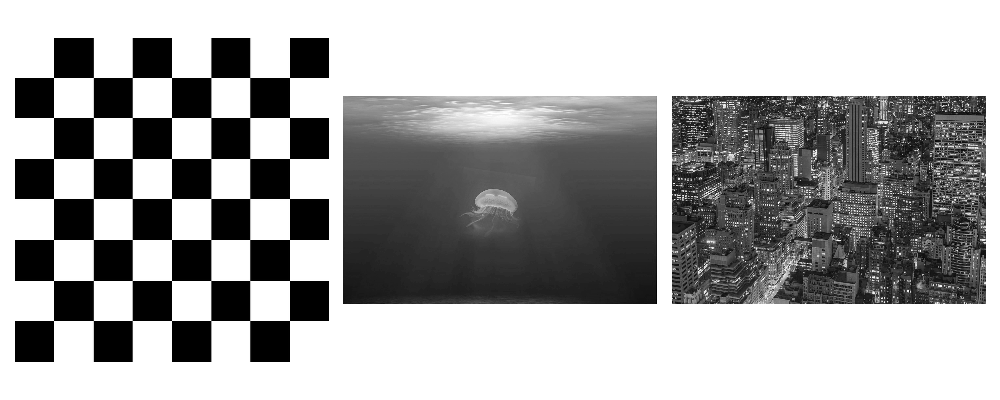
\includegraphics[width=1.0\linewidth]{../figs/original_img.png}
\end{figure}

\begin{figure}[H]
    \centering
    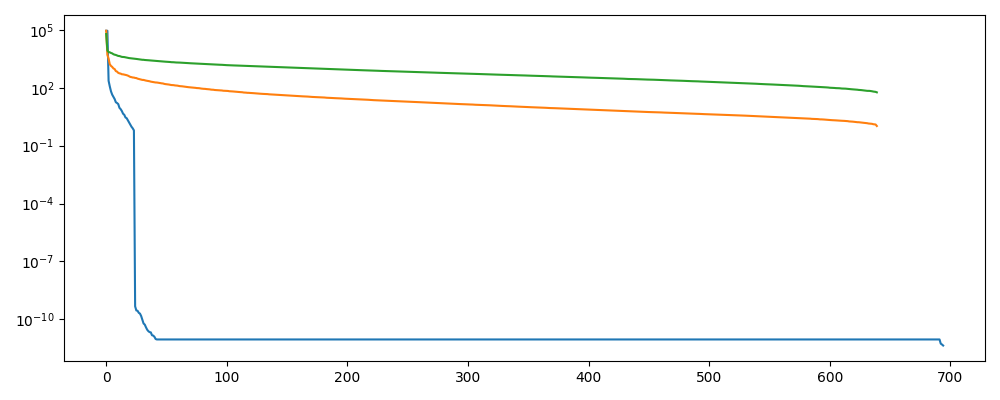
\includegraphics[width=1.0\linewidth]{../figs/singular_values.png}
\end{figure}


Below, the compressed versions of the images are plotted, for different number of singular values, $r$, and with calculated compression ratios. The chessboard looks indistiguishable already from $r=2$, and we can compress the image an impressive factor of $~50'000$ without losing information. The jellyfish starts looking good somewhere in the range $r=16-32$, where we have a compression ratio somewhere around $~300-1150$. For the new york image, we need around $r=64-128$ singular values for a good looking image, giving a compression ratio of only $~20-80$.

\begin{figure}[H]
    \centering
    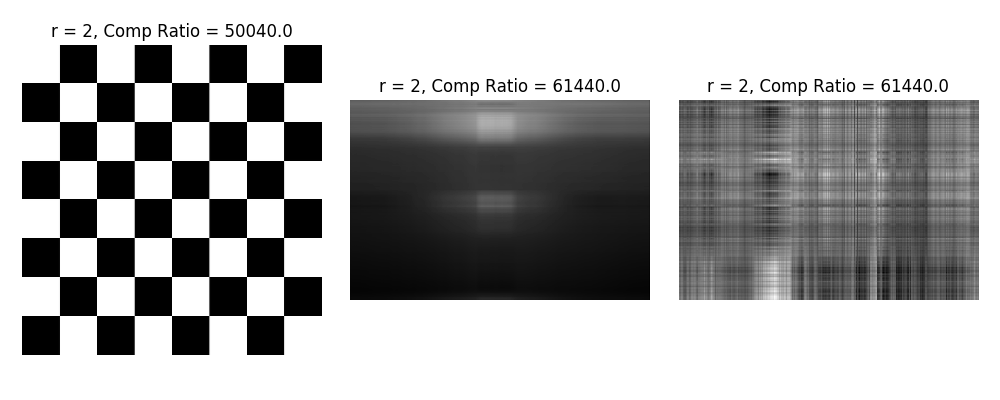
\includegraphics[width=1.0\linewidth]{../figs/img0.png}
    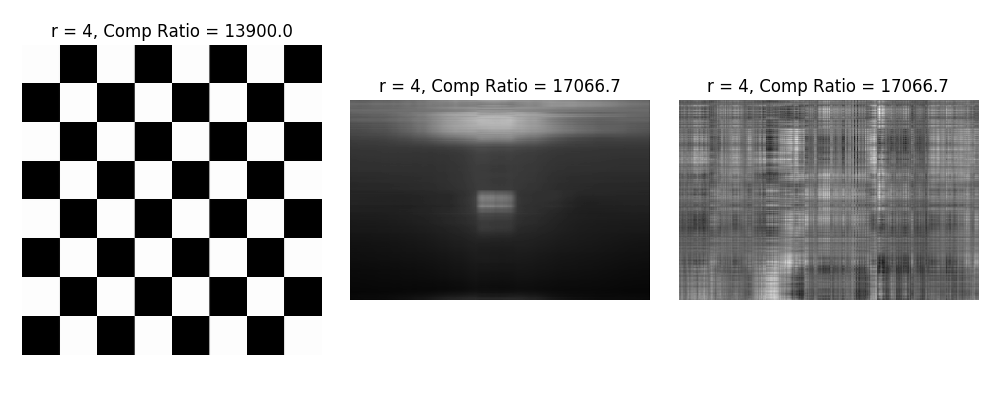
\includegraphics[width=1.0\linewidth]{../figs/img1.png}
    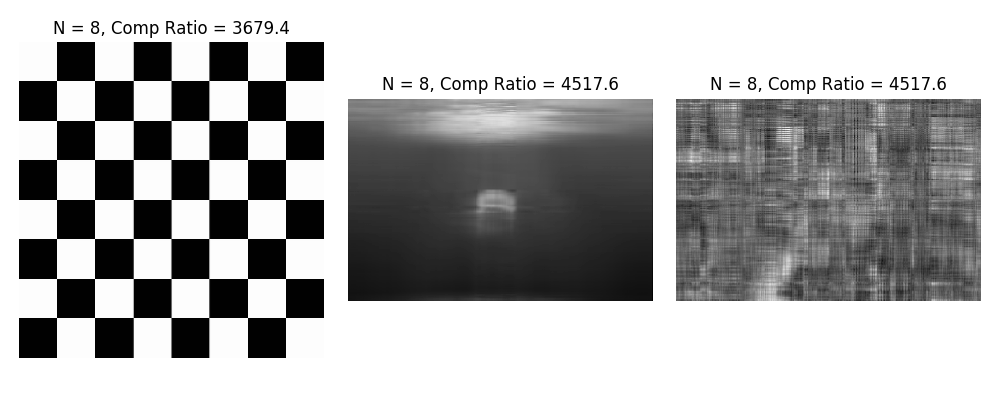
\includegraphics[width=1.0\linewidth]{../figs/img2.png}
\end{figure}

\begin{figure}[H]
    \centering
    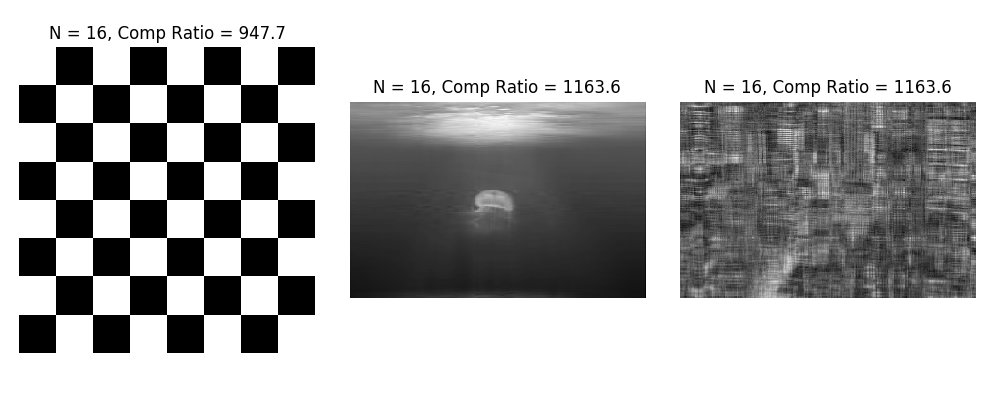
\includegraphics[width=1.0\linewidth]{../figs/img3.png}
    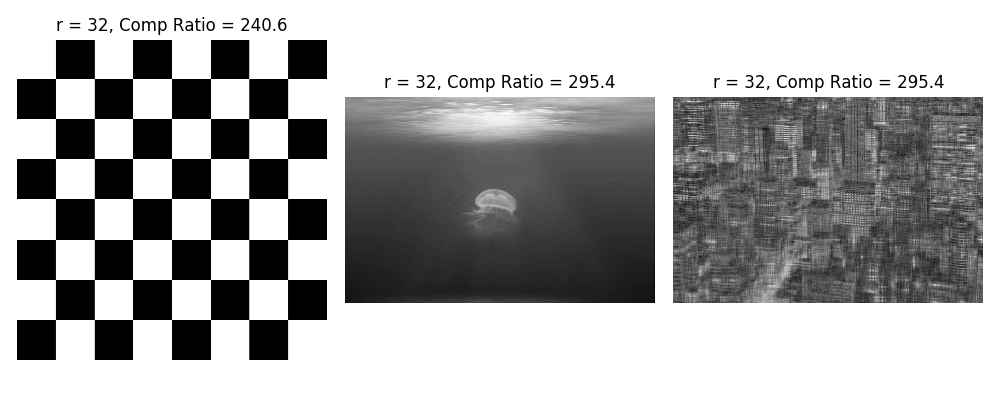
\includegraphics[width=1.0\linewidth]{../figs/img4.png}
    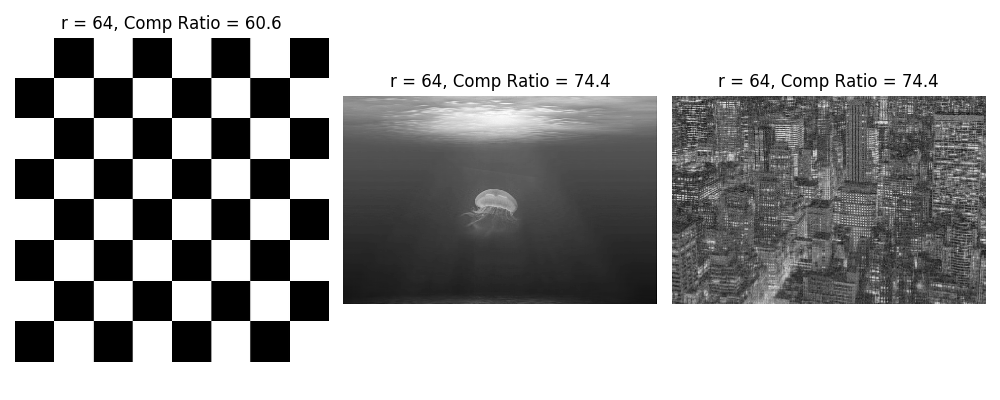
\includegraphics[width=1.0\linewidth]{../figs/img5.png}
\end{figure}

\begin{figure}[H]
    \centering
    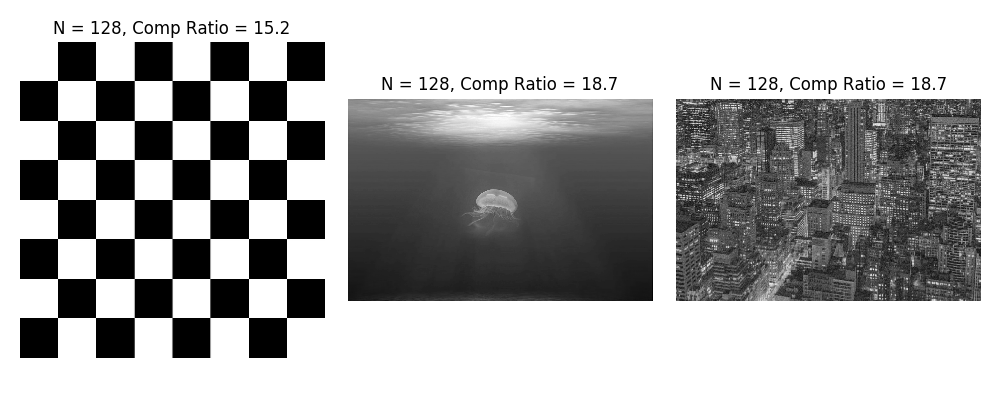
\includegraphics[width=1.0\linewidth]{../figs/img6.png}
    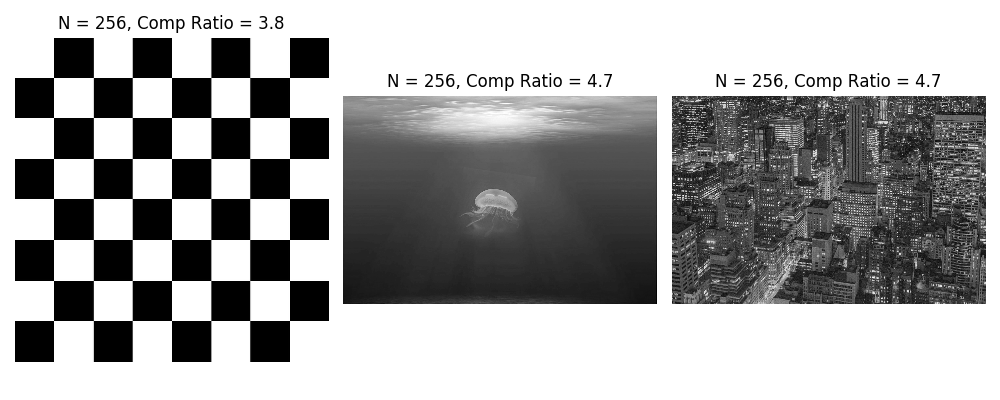
\includegraphics[width=1.0\linewidth]{../figs/img7.png}
    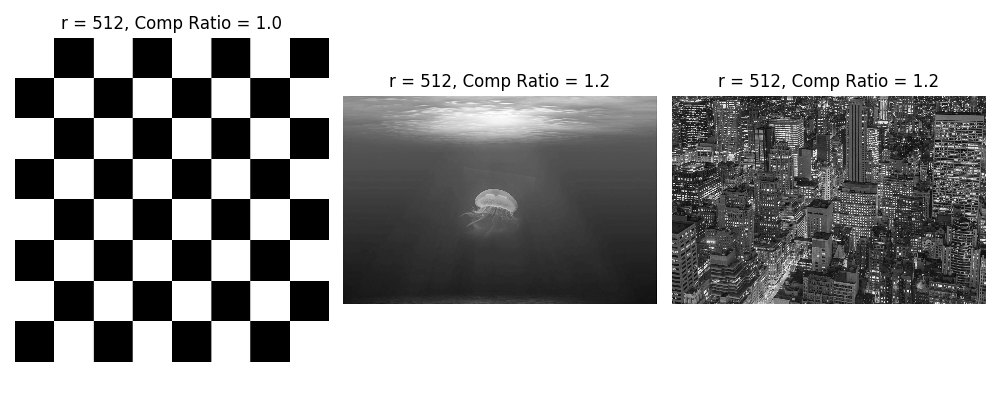
\includegraphics[width=1.0\linewidth]{../figs/img8.png}
\end{figure}


\section*{Appendix: Code}

\pagebreak

\lstinputlisting[language=Python, caption=oblig2.py, frame=full]{../src/oblig2.py}

\end{document}